\documentclass[utf8x]{G7-32} % Стиль (по умолчанию будет 14pt)
\usepackage[T2A]{fontenc}
\usepackage[russian]{babel}

\newcommand{\stend}{\textbf{Wb-demo-kit v.2}}

% Путь до папки с общими шаблонами
\newcommand{\pathToCommonFolder}{/home/denilai/Documents/repos/latex/Common}
\newcommand{\pathToScriptsFolder}{/home/denilai/Documents/repos/latex/scripts}

\sloppy

\usepackage{listings}

% Настройки стиля ГОСТ 7-32
% Для начала определяем, хотим мы или нет, чтобы рисунки и таблицы нумеровались в пределах раздела, или нам нужна сквозная нумерация.
\EqInChapter % формулы будут нумероваться в пределах раздела
\TableInChapter % таблицы будут нумероваться в пределах раздела
\PicInChapter % рисунки будут нумероваться в пределах раздела

% Добавляем гипертекстовое оглавление в PDF
\usepackage[
bookmarks=true, colorlinks=true, unicode=true,
urlcolor=black,linkcolor=black, anchorcolor=black,
citecolor=black, menucolor=black, filecolor=black,
]{hyperref}

%Величина «красной строки»


\usepackage[tableposition=top,singlelinecheck=false]{caption}
%\usepackage{subcaption}

\DeclareCaptionLabelFormat{gostfigure}{Рисунок #2}
\DeclareCaptionLabelFormat{gosttable}{Таблица #2}
\DeclareCaptionLabelSeparator{gost}{~---~}
% Можно разбивать длинные таблицы вручную, оформляя каждую как table. В этом случае для продолжений таблицы нужно создать отдельный стиль заголовка
\DeclareCaptionLabelFormat{continued}{Продолжение таблицы~#2}
\captionsetup*[ContinuedFloat]{labelformat=continued}
\captionsetup{labelsep=gost}
\captionsetup*[figure]{labelformat=gostfigure, justification=centering,font={small, bf}}  % выравнивание по центру
\captionsetup*[table]{hangindent=-10pt, indention=0pt,parindent=0pt,margin=0pt,labelformat=gosttable,justification=raggedright,font={small,it}}
\captionsetup*[lstlisting]{font={small, it}}

% Изменение начертания шрифта --- после чего выглядит таймсоподобно.
% apt-get install scalable-cyrfonts-tex

\IfFileExists{cyrtimes.sty}
    {
        \usepackage{cyrtimespatched}
    }
    {
        % А если Times нету, то будет CM...
    }

\usepackage{graphicx}   % Пакет для включения рисунков
%расположение графики
\graphicspath{{images/}{figures/}{screnshots/}{../images/}}  % папки с картинками

% С такими оно полями оно работает по-умолчанию:
% \RequirePackage[left=20mm,right=10mm,top=20mm,bottom=20mm,headsep=0pt]{geometry}
% Если вас тошнит от поля в 10мм --- увеличивайте до 20-ти, ну и про переплёт не забывайте:
\geometry{right=10mm}
\geometry{left=30mm}


% Пакет Tikz
\usepackage{tikz}
\usetikzlibrary{arrows,positioning,shadows}

% Произвольная нумерация списков.
\usepackage{enumerate}

% ячейки в несколько строчек
\usepackage{multirow}

% itemize внутри tabular
\usepackage{paralist,array}


% 8 Листинги

\usepackage{listings}

% Значения по умолчанию
\lstset{
  basicstyle= \footnotesize\ttfamily,
  breakatwhitespace=true,% разрыв строк только на whitespacce
  breaklines=true,       % переносить длинные строки
%   captionpos=b,          % подписи снизу -- вроде не надо
  inputencoding=koi8-r,
  numbers=left,          % нумерация слева
  numberstyle=\footnotesize,
  showspaces=false,      % показывать пробелы подчеркиваниями -- идиотизм 70-х годов
  showstringspaces=false,
  showtabs=false,        % и табы тоже
  stepnumber=1,
  tabsize=4,              % кому нужны табы по 8 символов?
  frame=single
}

% Стиль для псевдокода: строчки обычно короткие, поэтому размер шрифта побольше
\lstdefinestyle{pseudocode}{
  basicstyle=\small\ttfamily,
  keywordstyle=\color{black}\bfseries\underbar,
  language=Pseudocode,
  numberstyle=\footnotesize,
  commentstyle=\footnotesize\it\texttt
}

% Стиль для обычного кода: маленький шрифт
\lstdefinestyle{realcode}{
  basicstyle=\scriptsize,
  numberstyle=\footnotesize
}

% Стиль для коротких кусков обычного кода: средний шрифт
\lstdefinestyle{simplecode}{
  basicstyle=\footnotesize,
  numberstyle=\footnotesize
}

% Стиль для BNF
\lstdefinestyle{grammar}{
  basicstyle=\footnotesize,
  numberstyle=\footnotesize,
  stringstyle=\bfseries\ttfamily,
  language=BNF
}

% Определим свой язык для написания псевдокодов на основе Python
\lstdefinelanguage[]{Pseudocode}[]{Python}{
  morekeywords={each,empty,wait,do},% ключевые слова добавлять сюда
  morecomment=[s]{\{}{\}},% комменты {а-ля Pascal} смотрятся нагляднее
  literate=% а сюда добавлять операторы, которые хотите отображать как мат. символы
    {->}{\ensuremath{$\rightarrow$}~}2%
    {<-}{\ensuremath{$\leftarrow$}~}2%
    {:=}{\ensuremath{$\leftarrow$}~}2%
    {<--}{\ensuremath{$\Longleftarrow$}~}2%
}[keywords,comments]

% Свой язык для задания грамматик в BNF
\lstdefinelanguage[]{BNF}[]{}{
  morekeywords={},
  morecomment=[s]{@}{@},
  morestring=[b]",%
  literate=%
    {->}{\ensuremath{$\rightarrow$}~}2%
    {*}{\ensuremath{$^*$}~}2%
    {+}{\ensuremath{$^+$}~}2%
    {|}{\ensuremath{$|$}~}2%
}[keywords,comments,strings]

% Подписи к листингам на русском языке.
\renewcommand\lstlistingname{\cyr\CYRL\cyri\cyrs\cyrt\cyri\cyrn\cyrg}
\renewcommand\lstlistlistingname{\cyr\CYRL\cyri\cyrs\cyrt\cyri\cyrn\cyrg\cyri}


% Полезные макросы листингов.
% Любимые команды
\newcommand{\Code}[1]{\textbf{#1}}


% Название работы в титуле
\newcommand{\workname}{Отчет по практическим работам 9-12}
% Название дисциплины в титуле
\newcommand{\discipline}{Технологические основы Интернета вещей}
% Название кафедры в титуле
\newcommand{\kafedra}{Кафедра Математического обеспечения и стандартизации информационных технологий}
% Тема работы в титуле
\newcommand{\theme}{}
% Должность преподавателя в титуле
\newcommand{\rang}{ассистент}

% ФИО студента в титуле
\newcommand{\studentfio}{К.~Ю.~Денисов}%\\Д.~Н.~Федосеев\\А.~М.~Сосунов}\\%К.~Ю.~Денисов\\%И.~А.~Кремнев
% ФИО преподавателя в титуле
\newcommand{\teacherfio}{Ю.~А.~Воронцов}


\usepackage{tabularx}


\usepackage{booktabs}
\newcolumntype{b}{X}
\newcolumntype{s}{>{\hsize=.5\hsize}X}
\newcommand{\heading}[1]{\multicolumn{1}{c}{#1}}

% установка размера шрифта для всего документа
%\fontsize{20pt}{18pt}\selectfont
\usepackage{extsizes} % Возможность сделать 14-й шрифт

% Вставка заготовки преамбулы
%% Этот шаблон документа разработан в 2014 году
% Данилом Фёдоровых (danil@fedorovykh.ru) 
% для использования в курсе 
% <<Документы и презентации в \LaTeX>>, записанном НИУ ВШЭ
% для Coursera.org: http://coursera.org/course/latex .
% Исходная версия шаблона --- 
% https://www.writelatex.com/coursera/latex/5.3

% В этом документе преамбула

% Для корректного использования русских символов в формулах
% пакеты hyperref и настройки, связанные с ним, стоит загуржать
% перед загрузкой пакета mathtext



% поддержка русских букв
% кодировка шрифта
%\usepackage[T2A]{fontenc} 
\usepackage{pscyr}

% использование ненумеровонного абзаца с добавлением его в содержаниеl

\newcommand{\anonsection}[1]{\section*{#1}\addcontentsline{toc}{section}{#1}}
\newcommand{\sectionunderl}[1]{\section*{\underline{#1}}}


% настройка окружения enumerate
\usepackage{enumitem}
\setlist{noitemsep}
\setlist[enumerate]{labelsep=*, leftmargin=1.5pc}

\usepackage{hyperref}

% сначала ставить \usepackage{extsizes} % Возможность сделать 14-й шрифт
% для корректной установки полей вставлять преамбулу следует в последнюю очередь (но перед дерективой замены \rmdefault)
\usepackage[top=20mm,bottom=25mm,left=35mm,right=20mm]{geometry} % Простой способ задавать поля

\hypersetup{				% Гиперссылки
	unicode=true,           % русские буквы в раздела PDF
	pdftitle={Заголовок},   % Заголовок
	pdfauthor={Автор},      % Автор
	pdfsubject={Тема},      % Тема
	pdfcreator={Создатель}, % Создатель
	pdfproducer={Производитель}, % Производитель
	pdfkeywords={keyword1} {key2} {key3}, % Ключевые слова
	colorlinks=true,       	% false: ссылки в рамках; true: цветные ссылки
	linkcolor=red,          % внутренние ссылки
	citecolor=black,        % на библиографию
	filecolor=magenta,      % на файлы
	urlcolor=blue           % на URL
}

%%% Работа с русским языком
\usepackage{cmap}					% поиск в PDF
\usepackage{mathtext} 				% русские буквы в формулах
\usepackage[T2A]{fontenc}			% кодировка
\usepackage[utf8]{inputenc}			% кодировка исходного текста
\usepackage[english,russian]{babel}	% локализация и переносы
\usepackage{indentfirst}
\frenchspacing

%для изменения названия списка иллюстраций
\usepackage{tocloft}


\renewcommand{\epsilon}{\ensuremath{\varepsilon}}
\renewcommand{\phi}{\ensuremath{\varphi}}
\renewcommand{\kappa}{\ensuremath{\varkappa}}
\renewcommand{\le}{\ensuremath{\leqslant}}
\renewcommand{\leq}{\ensuremath{\leqslant}}
\renewcommand{\ge}{\ensuremath{\geqslant}}
\renewcommand{\geq}{\ensuremath{\geqslant}}
\renewcommand{\emptyset}{\varnothing}

% Изменения параметров списка иллюстраций
\renewcommand{\cftfigfont}{Рисунок } % добавляем везде "Рисунок" перед номером
\addto\captionsrussian{\renewcommand\listfigurename{Список иллюстративного материала}}

\newcommand{\tm}{\texttrademark\ }
\newcommand{\reg}{\textregistered\ }


%%% Дополнительная работа с математикой
\usepackage{amsmath,amsfonts,amssymb,amsthm,mathtools} % AMS
\usepackage{icomma} % "Умная" запятая: $0,2$ --- число, $0, 2$ --- перечисление

%% Номера формул
%\mathtoolsset{showonlyrefs=true} % Показывать номера только у тех формул, на которые есть \eqref{} в тексте.
%\usepackage{leqno} % Нумереация формул слева

%% Свои команды
\DeclareMathOperator{\sgn}{\mathop{sgn}}

%% Перенос знаков в формулах (по Львовскому)
\newcommand*{\hm}[1]{#1\nobreak\discretionary{}
{\hbox{$\mathsurround=0pt #1$}}{}}


% отступ для первого абзаца главы или параграфа
%\usepackage{indentfirst}

%%% Работа с картинками
\usepackage{graphicx}  % Для вставки рисунков
\graphicspath{{images/}{screnshots/}}  % папки с картинками
\DeclareGraphicsExtensions{.pdf,.png,.jpg}
\setlength\fboxsep{3pt} % Отступ рамки \fbox{} от рисунка
\setlength\fboxrule{1pt} % Толщина линий рамки \fbox{}
\usepackage{wrapfig} % Обтекание рисунков текстом

%%% Работа с таблицами
\usepackage{array,tabularx,tabulary,booktabs} % Дополнительная работа с таблицами
\usepackage{longtable}  % Длинные таблицы
\usepackage{multirow} % Слияние строк в таблице

%%% Теоремы
\theoremstyle{plain} % Это стиль по умолчанию, его можно не переопределять.
\newtheorem{theorem}{Теорема}[section]
\newtheorem{proposition}[theorem]{Утверждение}

\theoremstyle{plain} % Это стиль по умолчанию, его можно не переопределять.
\newtheorem{work}{Практическая работа}[part]


 
 
\theoremstyle{definition} % "Определение"
\newtheorem{corollary}{Следствие}[theorem]
\newtheorem{problem}{Задача}[section]
 
\theoremstyle{remark} % "Примечание"
\newtheorem*{nonum}{Решение}



%%% Программирование
\usepackage{etoolbox} % логические операторы

%%% Страница

%	\usepackage{fancyhdr} % Колонтитулы
% 	\pagestyle{fancy}
%   \renewcommand{\headrulewidth}{0pt}  % Толщина линейки, отчеркивающей верхний колонтитул
% 	\lfoot{Нижний левый}
% 	\rfoot{Нижний правый}
% 	\rhead{Верхний правый}
% 	\chead{Верхний в центре}
% 	\lhead{Верхний левый}
%	\cfoot{Нижний в центре} % По умолчанию здесь номер страницы

\usepackage{setspace} % Интерлиньяж
\onehalfspacing % Интерлиньяж 1.5
%\doublespacing % Интерлиньяж 2
%\singlespacing % Интерлиньяж 1

\usepackage{lastpage} % Узнать, сколько всего страниц в документе.

\usepackage{soul} % Модификаторы начертания


\usepackage[usenames,dvipsnames,svgnames,table,rgb]{xcolor}


\usepackage{csquotes} % Еще инструменты для ссылок

%\usepackage[style=authoryear,maxcitenames=2,backend=biber,sorting=nty]{biblatex}

\usepackage{multicol} % Несколько колонок

\usepackage{tikz} % Работа с графикой
\usepackage{pgfplots}
\usepackage{pgfplotstable}

% модуль для вставки рыбы
\usepackage{blindtext}

\usepackage{listings}
\usepackage{color}


% для поворота отдельной страницы. Использовать окружение \landscape
\usepackage{pdflscape} 
\usepackage{rotating} 


\definecolor{mygreen}{rgb}{0,0.6,0}
\definecolor{mygray}{rgb}{0.5,0.5,0.5}
\definecolor{mymauve}{rgb}{0.58,0,0.82}


% пример импорта файла
%\lstinputlisting{/home/denilai/repomy/conf/distributions}

\lstset{
	language=Python,
	basicstyle=\footnotesize,        % the size of the fonts that are used for the code
	numbers=left,                    % where to put the line-numbers; possible values are (none, left, right)
	numbersep=5pt,                   % how far the line-numbers are from the code
	numberstyle=\tiny\color{mygray}, % the style that is used for the line-numbers
	stepnumber=2,                    % the step between two line-numbers. If it's 1, each line will be numbered
	% Tab - 2 пробела
	tabsize=2,    
	% Автоматический перенос строк
	breaklines=true,
	frame=single,
	breakatwhitespace=true,
	title=\lstname 
}



\author{Кирилл Денисов}
\title{Лабораторная работа №1}
\date{\today}

\newcommand{\withouttheme}{1}

%если нужна тема работы в отчете, то указать в скобках что-либо, иначе оаставить пустым
%\renewcommand{\withouttheme}{}
%если нужна дата представления отчета, то указать в скобках что-либо
%\renewcommand{\withoutsubmissiondate}{1}

% установка полуторного интервала
% \usepackage{setspace}  
% \onehalfspacing

% использовать Times New Roman
\renewcommand{\rmdefault}{ftm}


\newcommand{\tb}{ThingsBoard~}

\begin{document}
	\thispagestyle{empty}
	% Вставка первого титульного листа
	% Есть две версии титульного листа - одиночный (titul) и групповой (titulAll)
	%\newcommand{\withouttheme}{} добавить эту переменную для определения, нужна ли тема
%     {} - нужна
%    {1} - не нужна

%\newcommand{\withoutsubmissiondate}{} добавить эту переменную для определения, нужен ли срок предоставления отчета
%     {} - нужен
%    {1} - не нужен

\renewcommand{\studentfio}{К.~Ю.~Денисов\\
				& & \hfill И.~А.~Кремнев \\
				& & \hfill А.~М.~Сосунов\\
				& & \hfill Д.~Н.~Федосеев}

\begin{center}
	\begin{figure}[h!]
		\begin{center}
			%\vspace{10ex}
			
\includegraphics[width=0.17\linewidth]{\pathToCommonFolder/gerb}
			%\caption{}\label{pic:first}
			%	\vspace{5ex}
		\end{center}	
	\end{figure}
 	\small	МИНОБРНАУКИ РОССИИ \\
Федеральное государственное бюджетное образовательное учреждение\\
высшего профессионального образования\\
	\normalsize					
	\textbf{«МИРЭА – Российский технологический университет»\\
		РТУ МИРЭА}\\
	\noindent\rule{1\linewidth}{1pt}\\
	Институт информационных технологий\\ %\vspace{2ex}
	\kafedra\\
	\vspace{3ex}
	\large \textbf{\workname}  \\
	%\vspace{1ex}
	по дисциплине\\ «\discipline» \\
	\vspace{3ex}
	\if \withouttheme
	\textbf{Тема работы:}\\ <<\theme>>
	\fi
	\vspace{6ex}
	\small
	\begin{table}[h!]
		\begin{tabular}{lp{0.55\linewidth}l}
			\textbf{Выполнили:} & студенты группы ИВБО-02-19 & \\ 
			& & \hfill \studentfio \\%Д.~Н.~Федосеев\\%А.~М.~Сосунов\\%К.~Ю.~Денисов\\%И.~А.~Кремнев
			\textbf{Принял:} & \rang & \\
			& & \hfill \teacherfio\\
		\end{tabular}
	\end{table}

	\normalsize
	
	\vfill
	Москва 2021
	
\end{center}
	\newpage
	\tableofcontents
	\newpage
	%\listoftables

\normalsize

\section{Практическая работа №9.\\Знакомство с облачными платформами IoT}
\subsection{Регистрация на платформе \tb}

\tb имеет тестовый сервер в сборке Community Edition для проверки доступных
функций платформы и тестирования своих приложений. Для регистрации на платформе
необходимо перейти по данной  \href{https://demo.\tb.io/signup}{ссылке}.

Зарегистрируемся на платформе \tb для выполнения данных практических работ.

\subsection{Создание виртуальных устройств в облаке}

Создадим в облаке следующие виртуальные устройства для получения данных:


\begin{enumerate}
	\item Датчик качества воздуха;
	\item Датчик освещенности;
	\item Датчик напряжения.
\end{enumerate}

Создадим для каждого устройства свой профиль (виртуальное устройство), соответствующий передаваемым на
устройство данным. В качестве протокола для профилей устройств используем \textbf{MQTT} (см. Рисунок \ref{fig:task9-create},\ref{fig:task9-create2}).
% TODO: \usepackage{graphicx} required
\begin{figure}[h!]
	\centering
	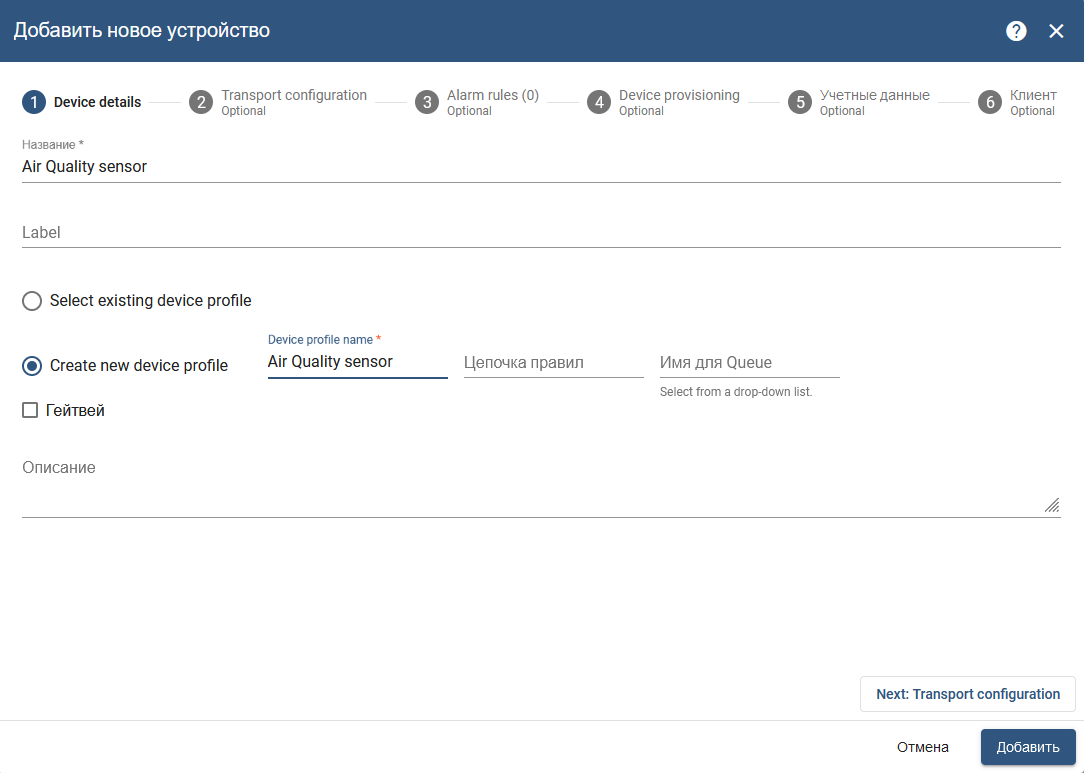
\includegraphics[width=0.7\linewidth]{images/task9-create}
	\caption{Создание устройства на платформе \tb}
	\label{fig:task9-create}
\end{figure}

\begin{figure}[h!]
	\centering
	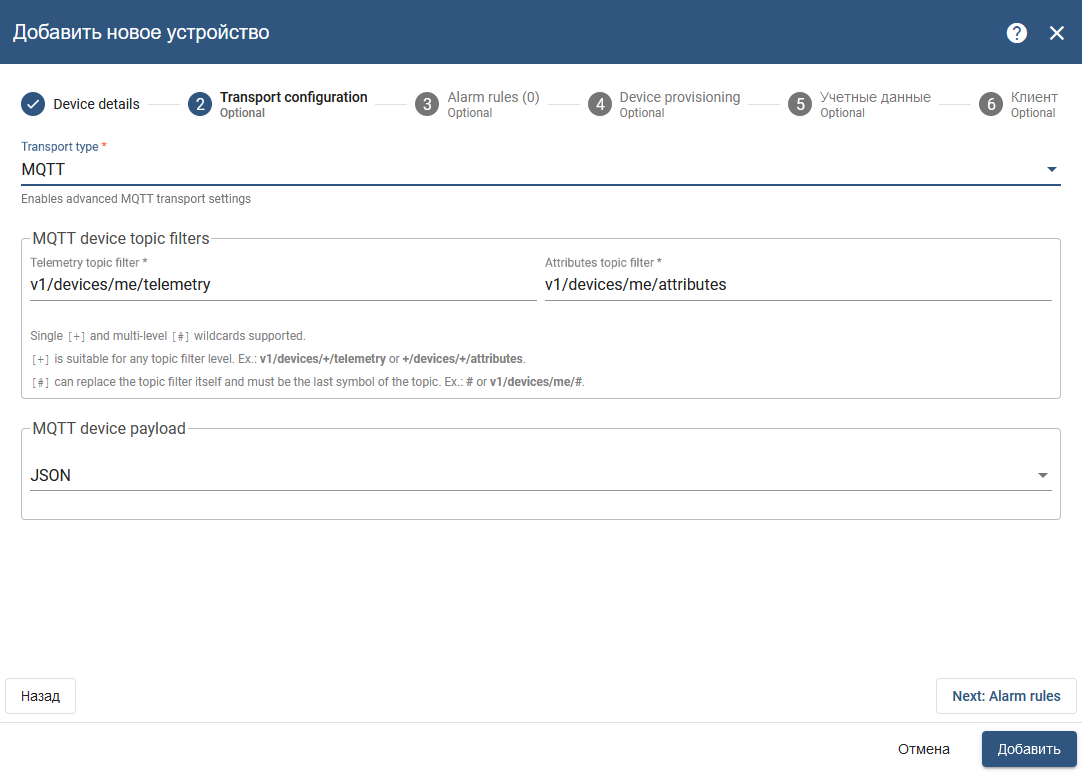
\includegraphics[width=0.7\linewidth]{images/task9-create2}
	\caption{Настройка устройства на платформе \tb}
	\label{fig:task9-create2}
\end{figure}

\subsection{Отправка данных в облако}

Выполним передачу тестовых данных в каждое из созданных устройств, список которых приведен на Рисунке \ref{fig:devices}.

% TODO: \usepackage{graphicx} required
\begin{figure}[h!]
	\centering
	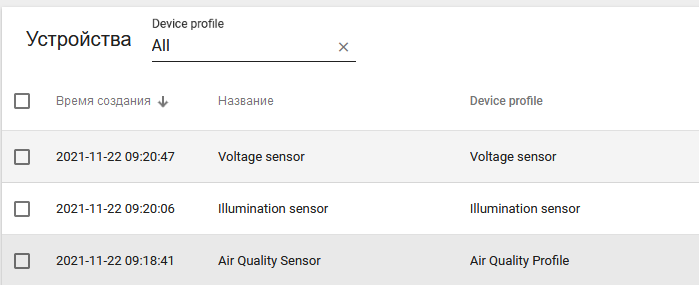
\includegraphics[width=0.7\linewidth]{images/devices}
	\caption{Список зарегистрированных устройств}
	\label{fig:devices}
\end{figure}

Приведем команду, с помощью которой осуществляется процесс ответа на сообщение с телеметрией в топик устройства с параметром "motion" (см. Рисунок (см. Рисунок \ref{fig:send}).

\begin{figure}[h!]
	\centering
	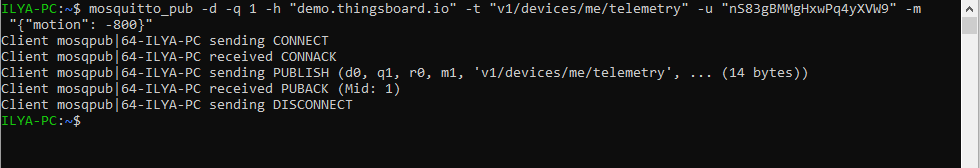
\includegraphics[width=0.7\linewidth]{images/send}
	\caption{Отправка данных на устройства}
	\label{fig:send}
\end{figure}

После отправки, тестовые данные отображаются в веб-интерфейсе платформы \tb в виде представленном на Рисунках \ref{fig:voltagedata}--\ref{fig:airqualitydata}. 
% TODO: \usepackage{graphicx} required
\begin{figure}[h!]
	\centering
	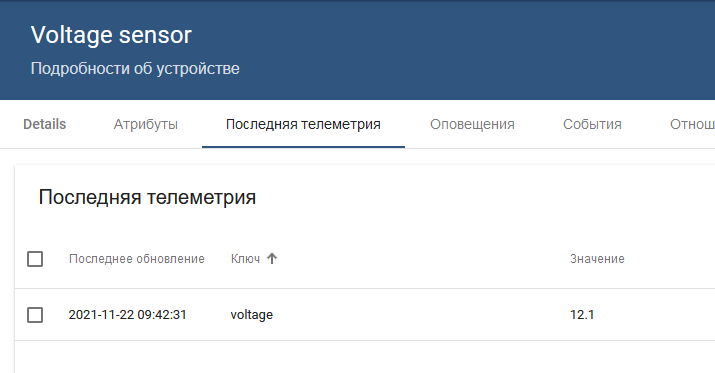
\includegraphics[width=0.7\linewidth]{images/VoltageData}
	\caption{Данные с датчика напряжения}
	\label{fig:voltagedata}
\end{figure}
% TODO: \usepackage{graphicx} required
\begin{figure}[h!]
	\centering
	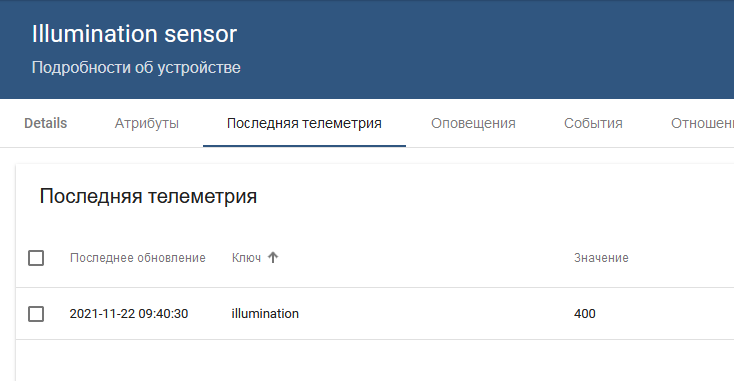
\includegraphics[width=0.7\linewidth]{images/IlluminationData}
	\caption{Данные с датчика освещения}
	\label{fig:illuminationdata}
\end{figure}
% TODO: \usepackage{graphicx} required
\begin{figure}[h!]
	\centering
	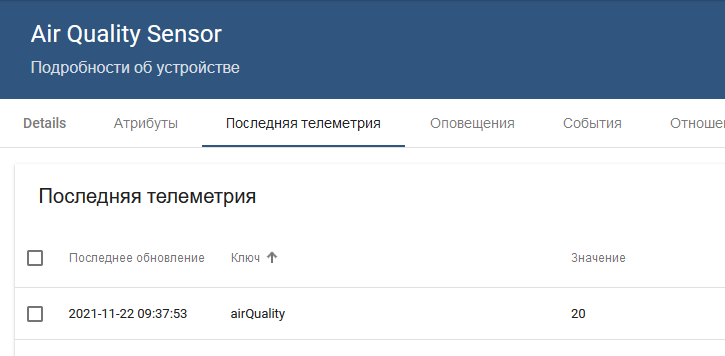
\includegraphics[width=0.7\linewidth]{images/airQualityData}
	\caption{Данные с датчика качества воздуха}
	\label{fig:airqualitydata}
\end{figure}


Данные соответствуют типу устройства и передаются при помощи утилиты \texttt{mosquito\_pub}.

\newpage

\section{Дополнительное задание практической работы №9}
\subsection{Выбор облачного решения}

В качестве облачного решения была выбрана платформа ThingsBoard. Данный выбор был сделан по следующим причинам:
\begin{itemize}
	\item Понятный пользовательский интерфейс;
	\item Популярность платформы;
	\item Возможность установить платформу локально или использовать готовую облачную среду.
\end{itemize}


\subsection{Реализация отправки данных}

Реализуем отправку данных с программного эмулятора реального физического устройства в облачную платформу ThingsBoard. Приведем листинг скрипта на языке программирования Python:

\lstinputlisting{\pathToScriptsFolder/dop9-publish.py}

В результате запуска данного скрипта происходит соединение с MQTT-брокером, создание экземпляра класса Client для MQTT-брокера, с последнующей передачей данных в облако (см. Рисунки \ref{fig:dop9-send},  \ref{fig:dop9-recieve}).


% TODO: \usepackage{graphicx} required
\begin{figure}[h!]
	\centering
	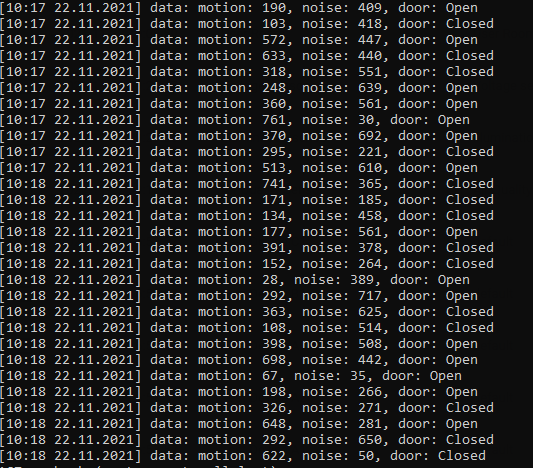
\includegraphics[width=0.6\linewidth]{images/dop9-send}
	\caption{Оправка телеметрических данных с устройств }
	\label{fig:dop9-send}
\end{figure}


% TODO: \usepackage{graphicx} required
\begin{figure}[h!]
	\centering
	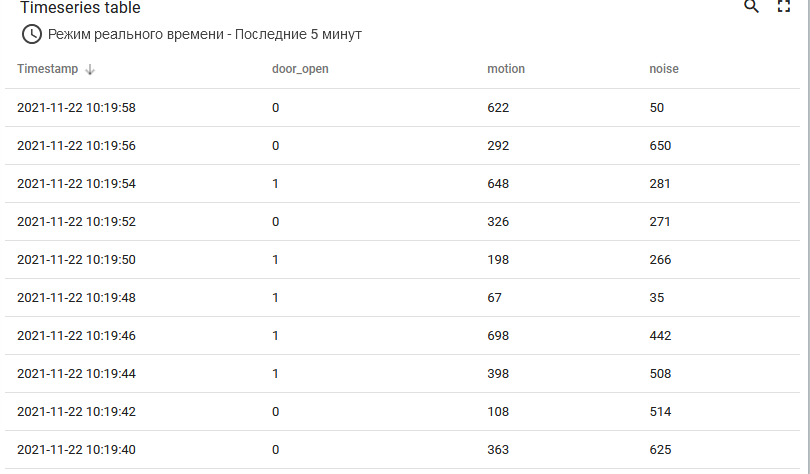
\includegraphics[width=0.6\linewidth]{images/dop9-recieve}
	\caption{Прием телеметрических данных облачной платформой}
	\label{fig:dop9-recieve}
\end{figure}
\hfill\newpage\hfill\newpage

\section{Практическая работа №10. \\Управление устройствами при помощи \\платформ Интернета вещей}

Реализуем следующие сценарии из практической работы №3 при помощи цепочек правил ThingsBoard.

\begin{enumerate}
	\item Включение и выключение вентилятора по датчику движения;
	\item Включение и выключения индикации зеленым и красным светом комбинированного датчика по кнопкам.
\end{enumerate}

\subsection{Реализация сценария управления вентилятором}
На платформе \tb создадим виртуальное устройство, которое будет прообразом реального вентилятора (см. Рисунок \ref{fig:dev}).

% TODO: \usepackage{graphicx} required
\begin{figure}[h!]
	\centering
	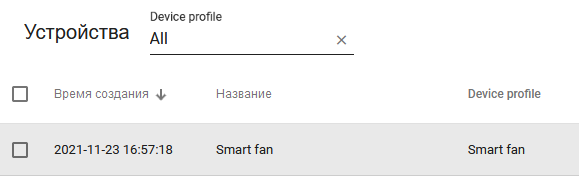
\includegraphics[width=0.5\linewidth]{images/dev}
	\caption{Виртуальный вентилятор}
	\label{fig:dev}
\end{figure}

Создадим цепочку правил для контроля за состоянием вентилятора. Когда значения, передаваемые датчиком движения превышают 700 условных единиц, вентилятор должен включаться. При уменьшении значения ниже 700, вентилятор должен выключаться. Приведенная на Рисунке \ref{fig:chains} цепочка правил описывает данный сценарий управления устройством.

% TODO: \usepackage{graphicx} required
\begin{figure}[h!]
	\centering
	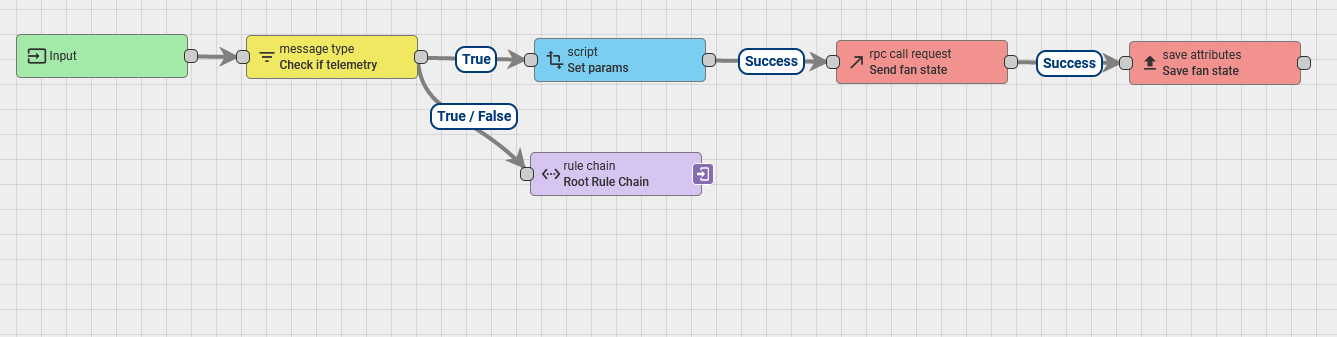
\includegraphics[width=0.6\linewidth]{images/chains}
	\caption{Цепочка правил для управления вентилятором}
	\label{fig:chains}
\end{figure}


\textbf{Узел формирования параметров вентилятора}

Узел трансформации данных при помощи скрипта позволяет переформировать объект,
содержащий в себе данные приходящего сообщения: его основную полезную нагрузку,
метаданные, а также тип сообщения.

Поведение узла описывается при помощи Java Script. Изначально в приходящей телеметрии
предполагается наличие параметра \texttt{motion}. На основании этого параметра
вычисляет новое состояние увлажнителя и формируется новый объект сообщения с этим
состоянием. 

Данный объект содержит в себе несколько свойств: \textit{method} --- это наименование
метода, при помощи которого можно будет идентифицировать необходимое действие на
устройстве, а также свойство \textit{params}, содержащее как раз состояние устройства, в которое
его необходимо привести. 

В дальнейшем этот объект будет отправлен на конечное
устройство для смены его состояния. Изменим тип события на событие загрузки
атрибутов устройства --- POST\_ATTRUBUTE\_REQUEST. Узел возвращает объект, содержащий в себе основное
сообщение, метаданные, а также тип сообщения. Полный код приведен ниже.


\lstinputlisting{\pathToScriptsFolder/fan_chain.js}

После реализации узла формирования параметров можно приступать к тестированию созданной цепочки. 

Подпишемся на топик запросов (v1/devices/me/rpc/request/+) созданного для данного
виртуального вентилятора. Воспользуемся для этого следующую командой:
\newpage
\begin{lstlisting}
	mosquitto_sub -v -h "demo.thingsboard.io" -t "v1/devices/me/rpc/request/+" -u "nS83gBMMgHxwPq4yXVW9"
\end{lstlisting}

После чего опубликуем сообщение с телеметрией в топик устройства с параметром
\texttt{motion}:

\begin{lstlisting}
mosquitto_pub -d -q 1 -h "demo.thingsboard.io" -t "v1/devices/me/telemetry" -u "nS83gBMMgHxwPq4yXVW9" -m "{"motion": 800}"
\end{lstlisting}

% TODO: \usepackage{graphicx} required
\begin{figure}[h!]
	\centering
	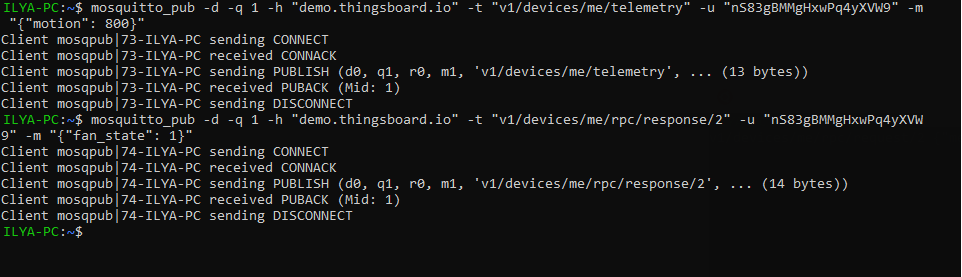
\includegraphics[width=0.6\linewidth]{images/t1-sender}
	\caption{Публикация сообщения с телеметрией вентилятора}
	\label{fig:t1-sender}
\end{figure}

Чтобы отправить ответ на опубликованный запрос на смену состояния, воспользуемся
также утилитой \texttt{mosquito\_pub}.

Для отправки ответа на созданный запрос необходимо послать сообщение в топик
\textit{v1/devices/me/rpc/response/2}. Воспользуемся для этого следующей командой:

\begin{lstlisting}
	mosquitto_pub -d -q 1 -h "demo.thingsboard.io" -t "v1/devices/me/rpc/response/2" -u "nS83gBMMgHxwPq4yXVW9" -m "{"fan_state": 1}"
\end{lstlisting}

После этого можно проверить в облаке поступившую телеметрию и аргументы устройства,
посланные в ответ на запрос. Результаты представлены на Рисунках \ref{fig:tel} и \ref{fig:attr}.

% TODO: \usepackage{graphicx} required
\begin{figure}[h!]
	\centering
	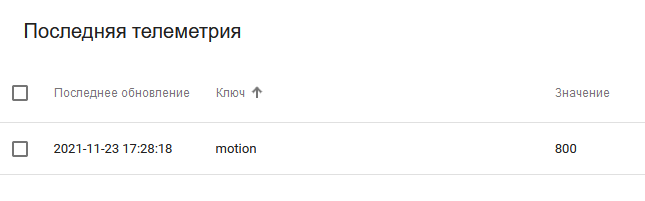
\includegraphics[width=0.6\linewidth]{images/tel}
	\caption{Телеметрия облачного устройства <<вентилятор>>}
	\label{fig:tel}
\end{figure}


\begin{figure}[h!]
	\centering
	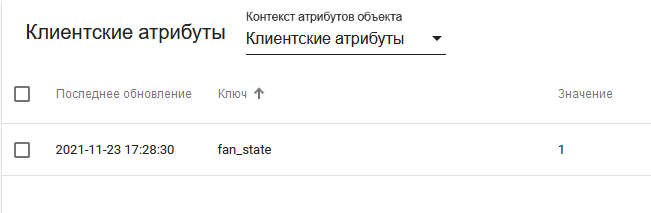
\includegraphics[width=0.6\linewidth]{images/attr}
	\caption{Атрибуты облачного устройства <<вентилятор>>}
	\label{fig:attr}
\end{figure}


\subsection{Реализация сценария управления лампами}


На платформе \tb создадим виртуальное устройство, которое будет прообразом реальных блока светодиодных ламп (см. Рисунок \ref{fig:dev-2}).


% TODO: \usepackage{graphicx} required
\begin{figure}[h!]
	\centering
	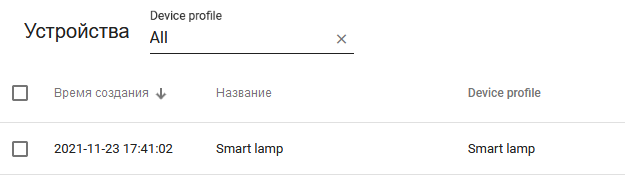
\includegraphics[width=0.5\linewidth]{images/dev-2}
	\caption{Виртуальный блок ламп}
	\label{fig:dev-2}
\end{figure}


Создадим цепочку правил для контроля за состоянием блока ламп. Световые индикаторы должны сигнализировать о включении и выключении комбинированного датчика. При включении датчика следует включить зеленую лампу, а при выключении --- красную. 

Приведенная на Рисунке \ref{fig:chains-2} цепочка правил описывает данный сценарий управления устройством.
% TODO: \usepackage{graphicx} required
\begin{figure}[h!]
	\centering
	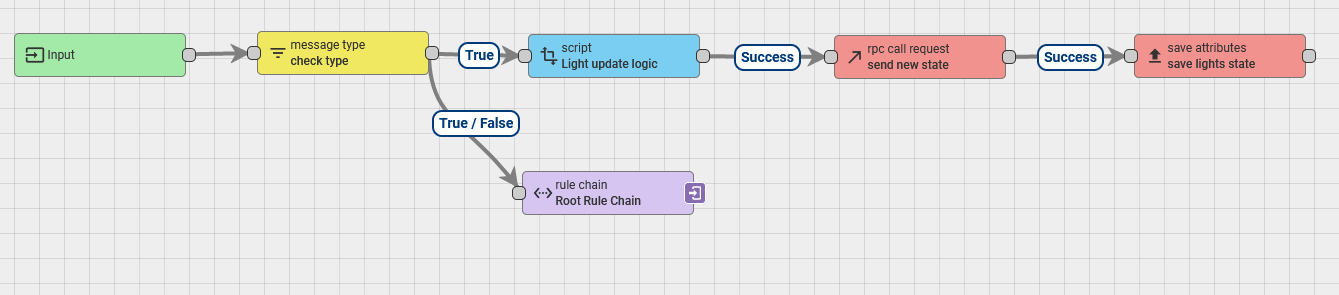
\includegraphics[width=0.6\linewidth]{images/chains-2}
	\caption{Цепочка правил для управления блоком ламп}
	\label{fig:chains-2}
\end{figure}


\textbf{Узел формирования параметров вентилятора}

Полный код, описывающий поведение узла формирования параметров блока умных ламп приведен ниже.


\lstinputlisting{\pathToScriptsFolder/light_chain.js}

После реализации узла формирования параметров можно приступать к тестированию созданной цепочки. 

Подпишемся на топик запросов (v1/devices/me/rpc/request/+) созданного для данного
виртуального контроллера. Воспользуемся для этого следующую командой:

\begin{lstlisting}
mosquitto_sub -v -h "demo.thingsboard.io" -t "v1/devices/me/rpc/request/+" -u "RxcWZHP60DTvKzcgWB0T"
\end{lstlisting}

После чего опубликуем сообщение с телеметрией в топик устройства с параметрами
\texttt{redButton} и \texttt{greenButton}:

\begin{lstlisting}
mosquitto_pub -d -q 1 -h "demo.thingsboard.io" -t "v1/devices/me/telemetry" -u "RxcWZHP60DTvKzcgWB0T" -m "{"redButton": 1, "greenButton": 0}"
\end{lstlisting}

% TODO: \usepackage{graphicx} required
\begin{figure}[h!]
	\centering
	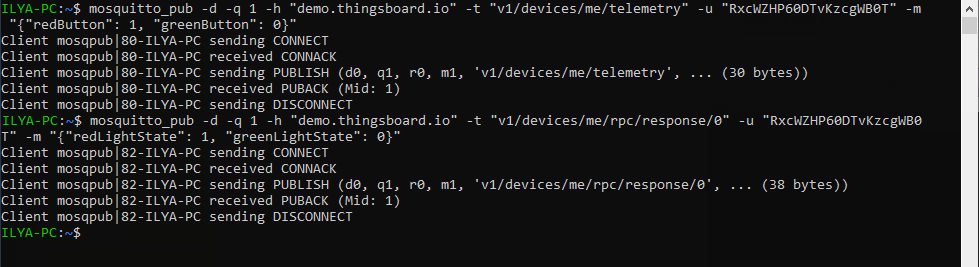
\includegraphics[width=0.6\linewidth]{images/t2-sender}
	\caption{Публикация сообщения с телеметрией блока ламп}
	\label{fig:t2-sender}
\end{figure}

Чтобы отправить ответ на опубликованный запрос на смену состояния, воспользуемся
также утилитой \texttt{mosquito\_pub}.

Для отправки ответа на созданный запрос необходимо послать сообщение в топик
\textit{v1/devices/me/rpc/response/2}. Воспользуемся для этого следующей командой:

\begin{lstlisting}
mosquitto_pub -d -q 1 -h "demo.thingsboard.io" -t "v1/devices/me/rpc/response/2" -u "RxcWZHP60DTvKzcgWB0T" -m "{"redLightState": 1, "greenLightState": 0}"
\end{lstlisting}

После этого можно проверить в облаке поступившую телеметрию и аргументы устройства,
посланные в ответ на запрос. Результаты представлены на Рисунках \ref{fig:tel-2} и \ref{fig:attr-2}.

% TODO: \usepackage{graphicx} required
\begin{figure}[h!]
	\centering
	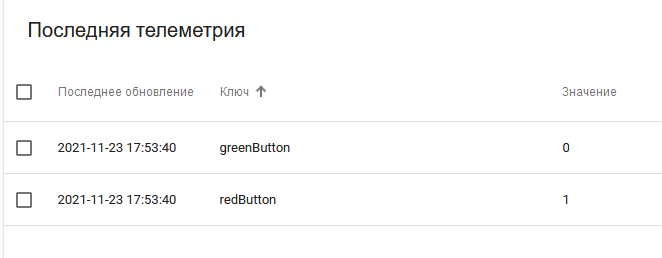
\includegraphics[width=0.6\linewidth]{images/tel-2}
	\caption{Телеметрия облачного устройства <<блок светодиодных ламп>>}
	\label{fig:tel-2}
\end{figure}


\begin{figure}[h!]
	\centering
	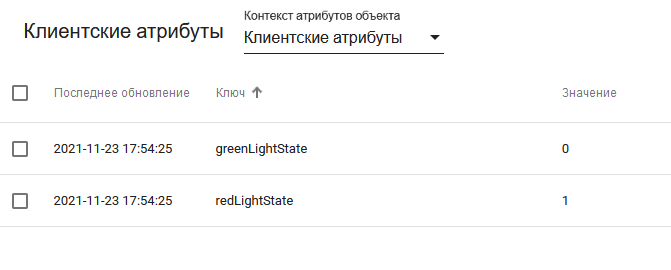
\includegraphics[width=0.6\linewidth]{images/attr-2}
	\caption{Атрибуты облачного устройства <<блок светодиодных ламп>>}
	\label{fig:attr-2}
\end{figure}


\section{Дополнительное задание практической работы № 10}

\subsection*{Описание взаимодействия пользователя с интерфейсом}
Опишите взаимодействие пользователя с интерфейсом вашего решения при
помощи графической нотации, к примеру, use-case диаграмм. 

\subsection{Требования к интерфейсу пользователя}

Для разрабатываемого нами программного решения был выбран интерфейс telegram~--~бота. Взаимодействие с данным интерфейсом состоит в отправке текстовых сообщений в мессенджере и основано на принципе <<запрос-ответ>> --- данные предоставляются пользователю по требованию.

Для удобного взаимодействия с информационной системой данные должны предоставляться пользователю в графическом, табличном и текстовом виде. Это упросит взаимодействие с программным инструментом.


Следует реализовать возможность выбора отслеживаемого на данный момент датчика, регистрации нового датчика (прибора), получения сведений о состоянии измерительного прибора, получении текущей телеметрии и статистических данных.

Сведения о передаваемой датчиками телеметрии следует представлять в виде таблиц, графиков или структурированного текста. Также нужно предоставить пользователю возможность получать сведения о данных за определенный временной промежуток, проводить их агрегирование.



\subsection{Макеты интерфейса приложения}

После проведения анализа существующих решений было сформировано представление о том, как следует выстроить взаимодействие с пользователем. 

Пользователю предлагается набор команд, которые понимает telegram--бот, их список приведен над полем ввода. На каждую команду бот отвечает установленным образом, предоставляя пользователю информацию о состоянии элементов системы. 

Решения использующие аналогичный интерфейс взаимодействия приведены на Рисунках \ref{fig:drewb}--\ref{fig:wash}.


% TODO: \usepackage{graphicx} required
\begin{figure}[h!]
	\centering
	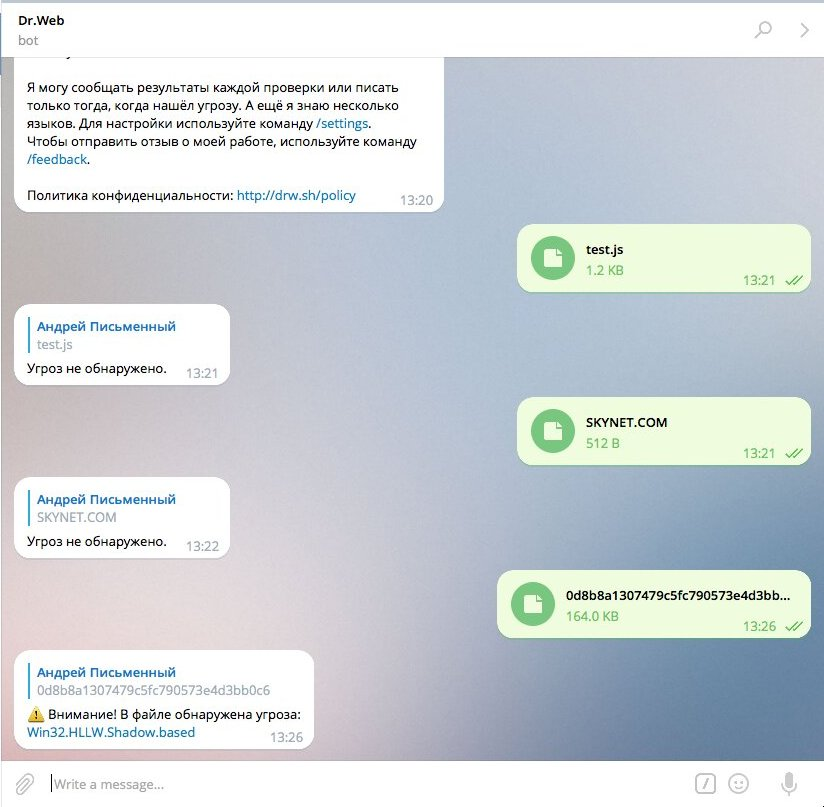
\includegraphics[width=0.5\linewidth]{images/mokups/drewb}
	\caption{Макет 1}
	\label{fig:drewb}
\end{figure}

\begin{figure}[h!]
	\centering
	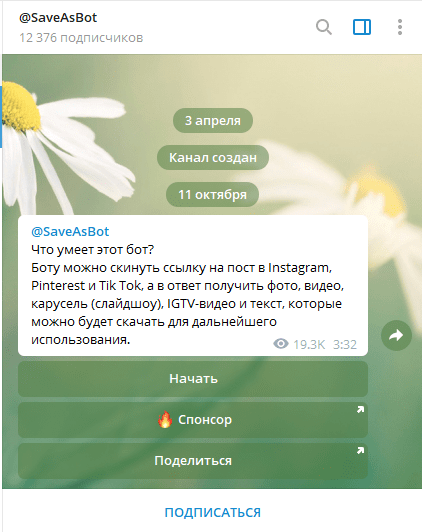
\includegraphics[width=0.5\linewidth]{images/mokups/saver}
	\caption{Макет 2}
	\label{fig:saver}
\end{figure}

% TODO: \usepackage{graphicx} required
\begin{figure}[h!]
	\centering
	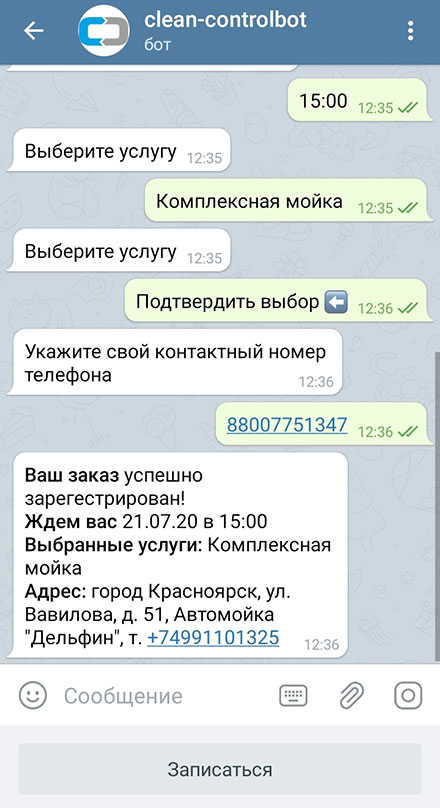
\includegraphics[width=0.5\linewidth]{images/mokups/wash}
	\caption{Макет 3}
	\label{fig:wash}
\end{figure}
% TODO: \usepackage{graphicx} required
\clearpage

\section{Практическая работа № 11. Реакции платформ Интернета вещей на приходящие данные}

\section{Добавление обработчиков тревожных сигналов}
Добавим в цепочки правил управления вентилятором тревогу при выходе приходящего параметра за допустимые границы.

Добавим в цепочки правил управления блоком светодиодов тревогу при отсутствии ожидаемого параметра в приходящем сообщении.
 
 
Также для обеих цепочек добавим тревогу при поступлении неверного ответа от физического устройства.



\end{document}




